% ============================================================
% Amazon-VT CFP 2026-2027 — 1-Page Abstract v4e
% AKG-E: Simulation-Grounded Validation
% Primary: AI Accelerated Science & Engineering
% Secondary: Agentic AI
% Format: IEEE 2-column
% ============================================================

\documentclass[conference, 10pt]{IEEEtran}

\usepackage[utf8]{inputenc}
\usepackage[T1]{fontenc}
\usepackage{graphicx}
\usepackage{hyperref}
\usepackage{microtype}
\usepackage{cite}
\usepackage{enumitem}
\setlist{nosep, leftmargin=1.5em, topsep=0.2em}
\usepackage{tikz}
\usetikzlibrary{positioning, arrows.meta, shapes.geometric, fit, calc}

\title{Agentic Knowledge Graphs for AI-Accelerated Engineering with Simulation-Grounded Validation}
\author{Jason Cusati \and Kereshmeh Afsari}
\date{}

% ============================================================
\begin{document}

\maketitle
\thispagestyle{empty}

\vspace{-1.5em}

\noindent\textbf{Primary Topic:} AI Accelerated Science \& Engineering \hfill
\textbf{Secondary:} Agentic AI

\vspace{0.5em}

AI-driven scientific breakthroughs increasingly rely on tightly coupling learned models with structured knowledge and simulation~\cite{Abramson2024AlphaFold3,Merchant2023GNoME}. Engineering disciplines face an analogous opportunity, yet large language models (LLMs) remain fundamentally misaligned with practice: they hallucinate physical quantities~\cite{Ji2023HallucinationSurvey}, fail to enforce constraints, and lack grounding in the structured ontologies and simulation feedback loops that govern real-world systems. While advances in knowledge-grounded generation---combining retrieval~\cite{Lewis2020RAG}, knowledge graphs~\cite{Edge2024GraphRAG}, and multi-source integration---improve factual consistency, they do not address the central \textit{application challenge}: no established methodology exists for validating AI-generated engineering outputs against physical laws and regulatory constraints~\cite{Oberkampf2010VVUQ}---a trust gap that blocks deployment.

This project proposes \textbf{Agentic Knowledge Graph Engineering (AKG-E)}, a domain-agnostic framework integrating knowledge-grounded reasoning with simulation-in-the-loop Verification, Validation, and Uncertainty Quantification (VVUQ). AKG-E applies three shared layers uniformly across engineering domains---with only the domain knowledge graph and simulator swapped: (1)~a \textit{domain ontology layer} encoding engineering KGs with entities, constraints, and physical laws; (2)~a \textit{simulation integration layer} exposing domain tools (Finite Element Analysis (FEA) solvers~\cite{Logg2012FEniCS}, digital twin microsimulators~\cite{Tao2019DigitalTwin}) as typed agent-callable interfaces; and (3)~a \textit{VVUQ validation layer} that verifies outputs against governing equations, quantifies uncertainty via Monte Carlo propagation through agent pipelines, and enforces regulatory constraints. Agents orchestrate across retrieval-augmented generation, structured graph queries, and simulation feedback, extending industry knowledge-grounding approaches (e.g., Amazon-scale KG systems~\cite{Yu2024COSMO}) with physics-based validation.

\begin{figure}[t]
    \centering
    \resizebox{\columnwidth}{!}{%
    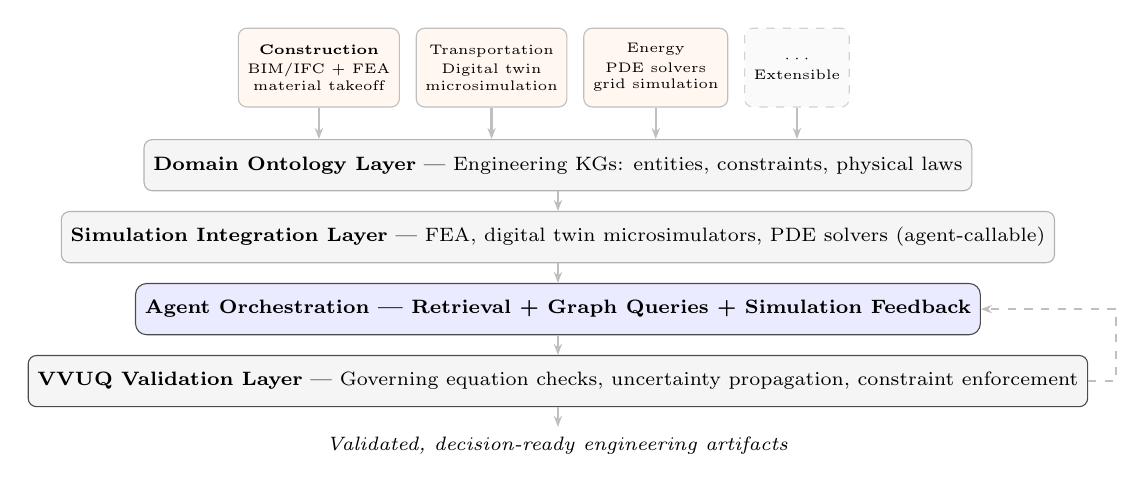
\begin{tikzpicture}[
        node distance=0.30cm and 0.20cm,
        layerbox/.style={rectangle, rounded corners=3pt, draw=gray!60, fill=gray!8, minimum width=7.8cm, minimum height=0.65cm, align=center, font=\scriptsize},
        dombox/.style={rectangle, rounded corners=3pt, draw=gray!50, fill=orange!6, minimum width=1.75cm, minimum height=1.0cm, align=center, font=\tiny},
        extbox/.style={rectangle, rounded corners=3pt, draw=gray!35, fill=gray!4, minimum width=1.05cm, minimum height=1.0cm, align=center, font=\tiny, dashed},
        agentbox/.style={rectangle, rounded corners=4pt, draw=black!70, fill=blue!8, minimum width=7.8cm, minimum height=0.65cm, align=center, font=\scriptsize\bfseries},
        arr/.style={-{Stealth[length=4pt]}, thick, gray!50},
    ]
        \node[dombox] (con) {\textbf{Construction}\\[1pt]BIM/IFC + FEA\\material takeoff};
        \node[dombox, right=0.20cm of con] (traf) {Transportation\\[1pt]Digital twin\\microsimulation};
        \node[dombox, right=0.20cm of traf] (energy) {Energy\\[1pt]PDE solvers\\grid simulation};
        \node[extbox, right=0.20cm of energy] (ext) {$\cdots$\\Extensible};

        \node[layerbox, below=0.40cm of $(con.south)!0.5!(ext.south)$] (onto) {\textbf{Domain Ontology Layer} --- Engineering KGs: entities, constraints, physical laws};

        \node[layerbox, below=0.25cm of onto] (sim) {\textbf{Simulation Integration Layer} --- FEA, digital twin microsimulators, PDE solvers (agent-callable)};

        \node[agentbox, below=0.25cm of sim] (agent) {Agent Orchestration --- Retrieval + Graph Queries + Simulation Feedback};

        \node[layerbox, below=0.25cm of agent, draw=black!70] (val) {\textbf{VVUQ Validation Layer} --- Governing equation checks, uncertainty propagation, constraint enforcement};

        \node[font=\scriptsize, below=0.25cm of val] (out) {\textit{Validated, decision-ready engineering artifacts}};

        \draw[arr] (con.south) -- (con.south |- onto.north);
        \draw[arr] (traf.south) -- (traf.south |- onto.north);
        \draw[arr] (energy.south) -- (energy.south |- onto.north);
        \draw[arr] (ext.south) -- (ext.south |- onto.north);
        \draw[arr] (onto) -- (sim);
        \draw[arr] (sim) -- (agent);
        \draw[arr] (agent) -- (val);
        \draw[arr] (val) -- (out);
        \draw[arr, dashed] (val.east) -- ++(0.35,0) |- (agent.east);
    \end{tikzpicture}
    }%
    \caption{\textbf{AKG-E Architecture.} Domain modules (Construction: primary; Transportation, Energy: extensions) plug into shared ontology, simulation, and VVUQ layers. The dashed feedback arrow represents iterative constraint-driven refinement.}
    \label{fig:framework}
    \vspace{-0.5em}
\end{figure}

This research pursues two questions: \textbf{RQ1:} How can VVUQ methodology be adapted to validate AI agent-generated engineering outputs, providing quantified uncertainty bounds and enforceable physical and regulatory constraints---evaluated against a curated benchmark of engineering tasks with known ground-truth solutions? \textbf{RQ2:} Does a domain-agnostic AKG-E architecture achieve measurable reductions in constraint violation rate and task success rate across engineering domains, relative to LLM-only and RAG-only baselines~\cite{Lewis2020RAG}? The intellectual merit lies in establishing \textit{a principled VVUQ methodology for agentic AI outputs}---a generalizable contribution that separates domain-specific knowledge from shared orchestration and validation logic. Core contributions include the VVUQ-agent integration methodology, a domain-agnostic pluggable architecture, and reproducible benchmarks for simulation-grounded agentic systems.

The primary pilot is \textbf{construction engineering}~\cite{Eastman2011BIM}: agents parse Building Information Modeling (BIM) models, perform material takeoff, invoke FEA~\cite{Logg2012FEniCS} for structural verification, and iterate under VVUQ gates until load constraints and building codes are satisfied. In \textbf{transportation engineering}, agents build and query digital twin models~\cite{Tao2019DigitalTwin} of traffic networks, optimize signal timing, and validate through microsimulation---with VVUQ verifying flow capacity and quantifying demand uncertainty. Expandability is explicit: the same three layers apply to energy and further domains by swapping only the domain KG and simulation interface; orchestration and VVUQ layers are reused unchanged. In practice, AKG-E transforms generative outputs into certified, decision-ready artifacts---reducing hallucinated designs, enforcing code compliance, and enabling principled human-in-the-loop thresholds. The framework targets deployment via Amazon Bedrock Knowledge Bases~\cite{AWSBedrockHybridSearch2024}, connecting AKG-E to AWS-scale engineering data pipelines and making it directly relevant to Amazon's applied AI and construction logistics workflows. We set a benchmark success criterion of $>$50\% constraint violation reduction versus unconstrained LLM baselines as an evaluation design target; deliverables include an open AKG-E framework, domain-adaptable KG templates, and VVUQ benchmarks for agentic systems.

\bibliographystyle{IEEEtran}
\bibliography{references}

\end{document}
